\documentclass{beamer}
\usefonttheme[onlymath]{serif}
\usepackage[T1]{fontenc}
\usepackage[utf8]{inputenc}
\usepackage[english]{babel}
\usepackage{amsmath}
\usepackage{amssymb}
\usepackage{amsthm}
\usepackage{gensymb}
\usepackage{parskip}
\usepackage{mathtools}
\usepackage{listings}
\usepackage{hyperref}
\usepackage{graphicx}
\usepackage{color}
\usepackage{enumerate}
\usepackage{tikz}
\usetikzlibrary{calc}
\usetikzlibrary{positioning}
\usetikzlibrary{angles}
\usetikzlibrary{shapes}
\usetikzlibrary{arrows}
\usepackage{verbatim}
\usepackage{multicol}
\usepackage{array}
\usepackage{minted}
\parskip 0pt


\DeclareMathOperator{\lcm}{lcm}
\newcommand\floor[1]{\left\lfloor#1\right\rfloor}
\newcommand\ceil[1]{\left\lceil#1\right\rceil}
\newcommand\abs[1]{\left|#1\right|}
\newcommand\p[1]{\left(#1\right)}
\newcommand\sqp[1]{\left[#1\right]}
\newcommand\cp[1]{\left\{#1\right\}}
\newcommand\norm[1]{\left\lVert#1\right\rVert}
\renewcommand\Im{\operatorname{Im}}
\renewcommand\Re{\operatorname{Re}}

\usetheme{metropolis}
\definecolor{dark yellow}{rgb} {0.6,0.6,0.0}
\definecolor{dark green}{rgb} {0.0,0.6,0.0}

\graphicspath{{myndir/}}

\title{More Dynamic Programming}
\author{Arnar Bjarni Arnarson}
\institute{\href{http://ru.is/td}{School of Computer Science} \\[2pt] \href{http://ru.is}{Reykjavík University}}
\titlegraphic{\hfill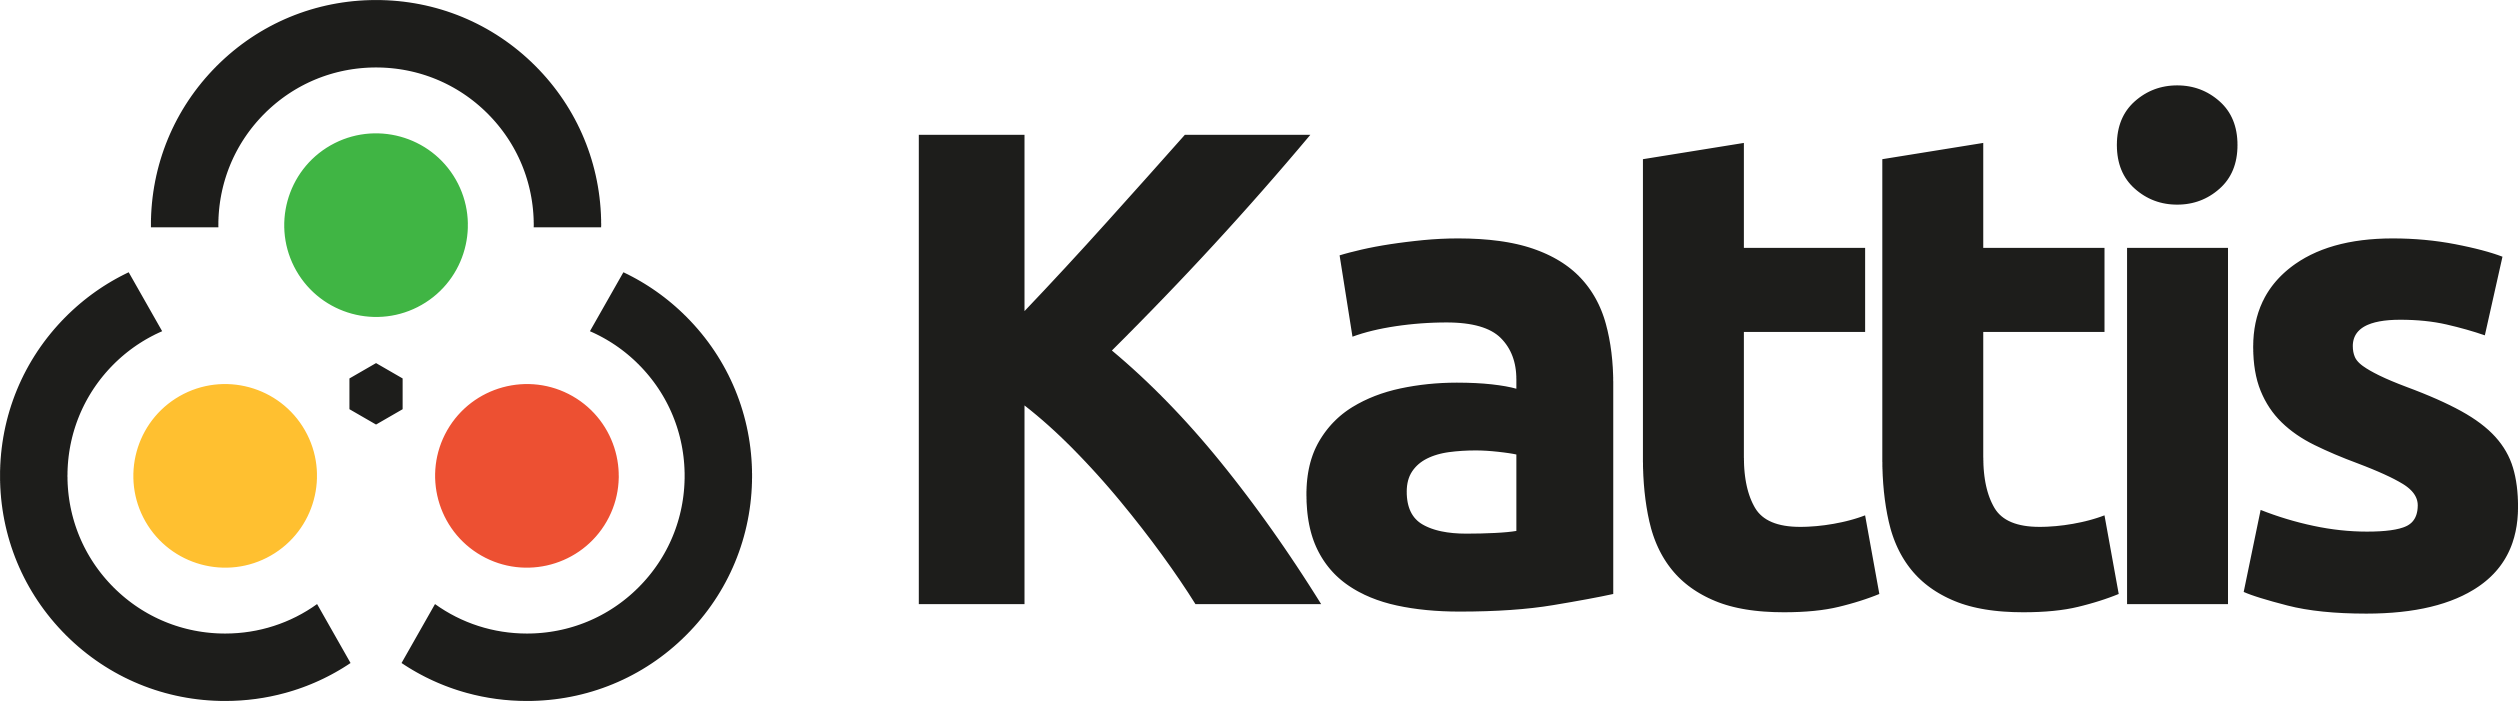
\includegraphics[height=0.6cm]{kattis}}

\begin{document}
\maketitle

\begin{frame}[plain]{What is dynamic programming?}
    \begin{itemize}
        \item A problem solving paradigm
        \item Similar in some respects to both divide and conquer and backtracking
        \vspace{5pt}
        \item Divide and conquer recap:
        \begin{itemize}
            \item Split the problem into \textit{independent} subproblems
            \item Solve each subproblem recursively
            \item Combine the solutions to subproblems into a solution for the given problem
        \end{itemize}
        \vspace{5pt}
        \item Dynamic programming:
        \begin{itemize}
            \item Split the problem into \textit{overlapping} subproblems
            \item Solve each subproblem recursively
            \item Combine the solutions to subproblems into a solution for the given problem
            \item \textit{Don't compute the answer to the same subproblem more than once}
        \end{itemize}
    \end{itemize}
\end{frame}

\begin{frame}[plain,fragile]{Dynamic programming formulation}
    \vspace{30pt}
    \begin{itemize}
        \item Formulate the problem in terms of smaller versions of the problem (recursively)
        \item Turn this formulation into a recursive function
        \item Memoize the function (remember results that have been computed)
    \end{itemize}
\end{frame}

\begin{frame}[plain,fragile]{Dynamic programming formulation}
    \begin{minted}[fontsize=\footnotesize]{cpp}
map<problem, value> memory;

value dp(problem P) {
    if (is_base_case(P)) {
        return base_case_value(P);
    }

    if (memory.find(P) != memory.end()) {
        return memory[P];
    }

    value result = some value;
    for (problem Q in subproblems(P)) {
        result = combine(result, dp(Q));
    }

    memory[P] = result;
    return result;
}
    \end{minted}
\end{frame}

\begin{frame}[plain]{The Fibonacci sequence}
    \vspace{5pt}
    \textit{The first two numbers in the Fibonacci sequence are 1 and 1. All
            other numbers in the sequence are defined as the sum of the previous two
            numbers in the sequence.}

    \vspace{5pt}
    \begin{itemize}
        \item Task: Find the $n$th number in the Fibonacci sequence
        \item Let's solve this with dynamic programming
    \end{itemize}

    \vspace{5pt}
    \begin{itemize}
        \item Formulate the problem in terms of smaller versions of the problem (recursively)
    \end{itemize}

    \begin{align*}
        \mathrm{fibonacci}(0) &= 0\\
        \mathrm{fibonacci}(1) &= 1\\
        \mathrm{fibonacci}(n) &= \mathrm{fibonacci}(n - 2) + \mathrm{fibonacci}(n - 1)
    \end{align*}
\end{frame}

\begin{frame}[plain,fragile]{The Fibonacci sequence}
    \begin{itemize}
        \item[2.] Turn this formulation into a recursive function
    \end{itemize}

    \begin{minted}[fontsize=\footnotesize]{cpp}
int fibonacci(int n) {
    if (n < 2) {
        return n;
    }

    int res = fibonacci(n - 2) + fibonacci(n - 1);

    return res;
}
    \end{minted}
\end{frame}

\begin{frame}[plain,fragile]{The Fibonacci sequence}
    \begin{itemize}
        \item What is the time complexity of this? \onslide<2->{Exponential, almost $O(2^n)$}
    \end{itemize}

    \begin{figure}
        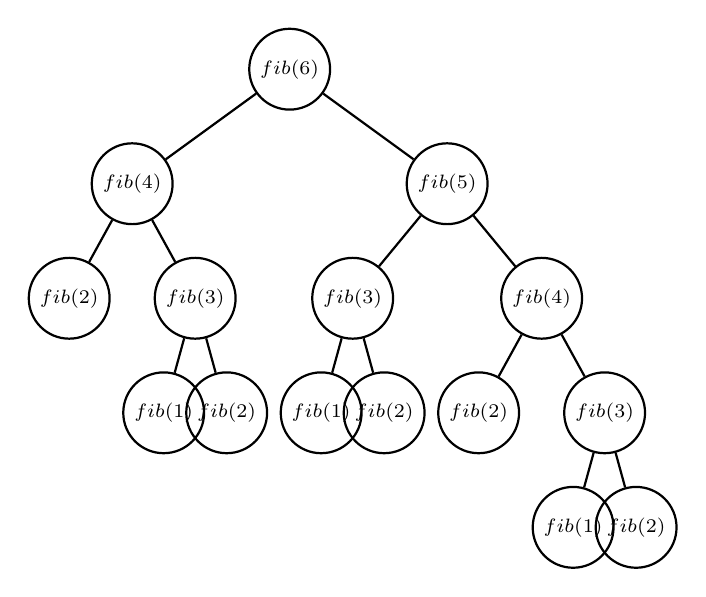
\begin{tikzpicture}[-,thick,%
  every node/.style={shape=circle,draw,thick},%
  level distance=0.5cm,%
  growth parent anchor={south}, nodes={anchor=north},%
  scale=0.8,%
]
\scriptsize
\node {$fib(6)$}
  [sibling distance=5cm]
  child {node {$fib(4)$}
    [sibling distance=2cm]
    child {node {$fib(2)$}
    }
    child {node {$fib(3)$}
      [sibling distance=1cm]
      child {node {$fib(1)$}
        [sibling distance=0.5cm]
      }
      child {node {$fib(2)$}
      }
    }
  }
  child {node {$fib(5)$}
    [sibling distance=3cm]
    child {node {$fib(3)$}
      [sibling distance=1cm]
      child {node {$fib(1)$}
        [sibling distance=0.5cm]
      }
      child {node {$fib(2)$}
          }
    }
    child {node {$fib(4)$}
      [sibling distance=2cm]
      child {node {$fib(2)$}
      }
      child {node {$fib(3)$}
        [sibling distance=1cm]
        child {node {$fib(1)$}
          [sibling distance=0.5cm]
        }
        child {node {$fib(2)$}
        }
      }
    }
  };
        \end{tikzpicture}
    \end{figure}
\end{frame}

\begin{frame}[plain,fragile]{The Fibonacci sequence}
    \begin{itemize}
        \item[3.] Memoize the function (remember results that have been computed)
    \end{itemize}

    \vspace{5pt}

    \begin{minted}[fontsize=\footnotesize]{cpp}
map<int, int> mem;

int fibonacci(int n) {
    if (n <= 2) {
        return 1;
    }

    if (mem.find(n) != mem.end()) {
        return mem[n];
    }

    int res = fibonacci(n - 2) + fibonacci(n - 1);

    mem[n] = res;
    return res;
}
    \end{minted}

\end{frame}

\begin{frame}[plain,fragile]{The Fibonacci sequence}
    \vspace{5pt}

    \begin{minted}[fontsize=\footnotesize]{cpp}
int mem[1000];
for (int i = 0; i < 1000; i++)
    mem[i] = -1;

int fibonacci(int n) {
    if (n <= 2) {
        return 1;
    }

    if (mem[n] != -1) {
        return mem[n];
    }

    int res = fibonacci(n - 2) + fibonacci(n - 1);

    mem[n] = res;
    return res;
}
    \end{minted}

\end{frame}

\begin{frame}[plain]{The Fibonacci sequence}
    \begin{itemize}
        \item What is the time complexity now?
        \vspace{5pt}
        \item We have $n$ possible inputs to the function: $1$, $2$, \ldots, $n$.
        \item Each input will either:
            \begin{itemize}
                \item be computed, and the result saved
                \item be returned from memory
            \end{itemize}
        \item Each input will be computed at most once
        \item Time complexity is $O(n \times f)$, where $f$ is the time complexity of computing an input if we assume that the recursive calls are returned directly from memory ($O(1)$)
        \item Since we're only doing constant amount of work to compute the answer to an input, $f = O(1)$
        \item Total time complexity is $O(n)$
    \end{itemize}
\end{frame}

\begin{frame}[plain]{Maximum sum}

    \vspace{10pt}

    \begin{itemize}
\item Given an array $\mathrm{arr}[0]$, $\mathrm{arr}[1]$, \ldots, $\mathrm{arr}[n-1]$ of integers, find the interval with the highest sum
    \end{itemize}

    \begin{center}
        \begin{tabular}{|c|c|c|c|c|c|c|}
            \hline
            -15 & \color<2->{blue}{8} & \color<2->{blue}{-2} & \color<2->{blue}{1} & \color<2->{blue}{0} & \color<2->{blue}{6} & -3 \\
            \hline
        \end{tabular}
    \end{center}

    \begin{itemize}
        \item<2-> The maximum sum of an interval in this array is $13$

        \item<3-> But how do we solve this in general?
            \begin{itemize}
        \item Easy to loop through all $\approx n^2$ intervals, and calculate their sums, but that is $O(n^3)$
        \item We could use our static range sum trick to get this down to $O(n^2)$
        \item Can we do better with dynamic programming?
            \end{itemize}
    \end{itemize}

\end{frame}

\begin{frame}[plain]{Maximum sum}

    \vspace{20pt}

    \begin{itemize}
        \item First step is to formulate this recursively
        \vspace{5pt}
        \item Let $\mathrm{max\_{}sum}(i)$ be the maximum sum interval in the range $0,\ldots,i$
        \vspace{5pt}
        \item Base case: $\mathrm{max\_{}sum}(0) = \mathrm{max}(0, arr[0])$
        \vspace{5pt}
        \item What about $\mathrm{max\_{}sum}(i)$?
        \item What does $\mathrm{max\_{}sum}(i-1)$ return?
        \item Is it possible to combine solutions to subproblems with smaller $i$ into a solution for $i$?
        \vspace{5pt}
        \item At least it's not obvious...
    \end{itemize}

\end{frame}

\begin{frame}[plain]{Maximum sum}

    \vspace{20pt}

    \begin{itemize}
        \item Let's try changing perspective
        \vspace{5pt}
    \item Let $\mathrm{max\_{}sum}(i)$ be the maximum sum interval in the range $0,\ldots,i$, \textit{that ends at $i$}
        \vspace{5pt}
        \item Base case: $\mathrm{max\_{}sum}(0) = arr[0]$
        \vspace{5pt}
    \item $\mathrm{max\_{}sum}(i) = \mathrm{max}(arr[i], arr[i] + \mathrm{max\_{}sum}(i - 1))$
        \vspace{15pt}
        \item Then the answer is just $\mathrm{max}_{\ 0 \leq i < n}\ \{\ \mathrm{max\_{}sum}(i)\ \}$
    \end{itemize}

\end{frame}

\begin{frame}[plain,fragile]{Maximum sum}
    \begin{itemize}
        \item Next step is to turn this into a function
    \end{itemize}

    \begin{minted}{cpp}
int arr[1000];

int max_sum(int i) {
    if (i == 0) {
        return arr[i];
    }

    int res = max(arr[i], arr[i] + max_sum(i - 1));

    return res;
}
    \end{minted}
\end{frame}

\begin{frame}[plain,fragile]{Maximum sum}
    \begin{itemize}
        \item Final step is to memoize the function
    \end{itemize}

    \begin{minted}[fontsize=\scriptsize]{cpp}
int arr[1000];
int mem[1000];
bool comp[1000];
memset(comp, 0, sizeof(comp));

int max_sum(int i) {
    if (i == 0) {
        return arr[i];
    }
    if (comp[i]) {
        return mem[i];
    }

    int res = max(arr[i], arr[i] + max_sum(i - 1));

    mem[i] = res;
    comp[i] = true;
    return res;
}
    \end{minted}
\end{frame}

\begin{frame}[plain,fragile]{Maximum sum}
    \begin{itemize}
        \item Then the answer is just the maximum over all interval ends
    \end{itemize}

    \begin{minted}[fontsize=\normalsize]{cpp}
int maximum = 0;
for (int i = 0; i < n; i++) {
    maximum = max(maximum, max_sum(i));
}

printf("%d\n", maximum);
    \end{minted}
\end{frame}

\begin{frame}[plain,fragile]{Maximum sum}
    \vspace{40pt}
    \begin{itemize}
        \item If you want to find the maximum sum interval in multiple arrays, remember to clear the memory in between
    \end{itemize}
\end{frame}

\begin{frame}[plain]{Maximum sum}
    \vspace{20pt}
    \begin{itemize}
        \item What about time complexity?
        \vspace{5pt}
        \item There are $n$ possible inputs to the function
        \item Each input is processed in $O(1)$ time, assuming recursive calls are $O(1)$
        \item Time complexity is $O(n)$
    \end{itemize}
\end{frame}

\begin{frame}[plain]{Coin change}
    \vspace{20pt}

    \begin{itemize}
\item Given an array of coin denominations $d_0$, $d_1$, \ldots, $d_{n-1}$,
            and some amount $x$: What is minimum number of coins needed to
            represent the value $x$?

        \item Remember the greedy algorithm for Coin change?
        \item It didn't always give the optimal solution, and sometimes it didn't even give a solution at all...

        \vspace{10pt}
        \item What about dynamic programming?
    \end{itemize}
\end{frame}

\begin{frame}[plain]{Coin change}
    \begin{itemize}
        \item First step: formulate the problem recursively
        \vspace{20pt}
\item Let $\mathrm{opt}(i,x)$ denote the minimum number of coins needed to represent the value $x$ if we're only allowed to use coin denominations $d_0$, \ldots, $d_i$
        \vspace{10pt}
        \item Base case: $\mathrm{opt}(i,x) = \infty$ if $x < 0$
        \item Base case: $\mathrm{opt}(i,0) = 0$
        \item Base case: $\mathrm{opt}(-1,x) = \infty$
        \vspace{10pt}
\item $\mathrm{opt}(i,x) = \mathrm{min} \left\{
	\begin{array}{l}
        1 + \mathrm{opt}(i, x - d_i) \\
        \mathrm{opt}(i-1, x)
	\end{array}
\right.$
    \end{itemize}
\end{frame}

\begin{frame}[plain,fragile]{Coin change}
    \begin{minted}[fontsize=\footnotesize]{cpp}
int INF = 100000;
int d[10];

int opt(int i, int x) {
    if (x < 0) return INF;
    if (x == 0) return 0;
    if (i == -1) return INF;

    int res = INF;
    res = min(res, 1 + opt(i, x - d[i]));
    res = min(res, opt(i - 1, x));

    return res;
}
    \end{minted}
\end{frame}

\begin{frame}[plain,fragile]{Coin change}
    \begin{minted}[fontsize=\footnotesize]{cpp}
int INF = 100000;
int d[10];
int mem[10][10000];
memset(mem, -1, sizeof(mem));

int opt(int i, int x) {
    if (x < 0) return INF;
    if (x == 0) return 0;
    if (i == -1) return INF;

    if (mem[i][x] != -1) return mem[i][x];

    int res = INF;
    res = min(res, 1 + opt(i, x - d[i]));
    res = min(res, opt(i - 1, x));

    mem[i][x] = res;
    return res;
}
    \end{minted}
\end{frame}

\begin{frame}[plain]{Coin change}
    \vspace{30pt}
    \begin{itemize}
        \item Time complexity?
        \item Number of possible inputs are $n \times x$
        \item Each input will be processed in $O(1)$ time, assuming recursive calls are constant
        \item Total time complexity is $O(n\times x)$
    \end{itemize}
\end{frame}

\begin{frame}[plain]{Coin change}
    \begin{itemize}
        \vspace{30pt}
        \item How do we know which coins the optimal solution used?
        \item We can store backpointers, or some extra information, to trace backwards through the states
        \item See example...
    \end{itemize}
\end{frame}

\begin{frame}[plain]{Longest increasing subsequence}
    \begin{itemize}
\item Given an array $a[0]$, $a[1]$, \ldots, $a[n-1]$ of integers, what is the length of the longest increasing subsequence?
    \vspace{3pt}
\item First, what is a subsequence?
\item If we delete zero or more elements from $a$, then we have a subsequence of $a$
    \vspace{3pt}
\item Example: $a = [5,1,8,1,9,2]$
    \vspace{3pt}
\item $[5,8,9]$ is a subsequence
\item $[1,1]$ is a subsequence
\item $[5,1,8,1,9,2]$ is a subsequence
\item $[]$ is a subsequence
\item $[8,5]$ is \textbf{not} a subsequence
\item $[10]$ is \textbf{not} a subsequence
    \end{itemize}
\end{frame}

\begin{frame}[plain]{Longest increasing subsequence}
    \begin{itemize}
\item Given an array $a[0]$, $a[1]$, \ldots, $a[n-1]$ of integers, what is the length of the longest increasing subsequence?
    \vspace{3pt}
\item An increasing subsequence of $a$ is a subsequence of $a$ such that the elements are in (strictly) increasing order
    \vspace{3pt}
\item $[5,8,9]$ and $[1,8,9]$ are the longest increasing subsequences of $a = [5,1,8,1,9,2]$

    \vspace{3pt}
\item How do we compute the length of the longest increasing subsequence?
\item There are $2^n$ subsequences, so we can go through all of them
\item That would result in an $O(n2^n)$ algorithm, which can only handle $n\leq 23$
    \vspace{3pt}
\item What about dynamic programming?

    \end{itemize}
\end{frame}

\begin{frame}[plain]{Longest increasing subsequence}
    \vspace{20pt}
    \begin{itemize}
\item Let $\mathrm{lis}(i)$ denote the length of the longest increasing subsequence of the array $a[0]$, $\ldots$, $a[i]$
    \vspace{5pt}
\item Base case: $\mathrm{lis}(0) = 1$
\item What about $\mathrm{lis}(i)$?
    \vspace{10pt}
\item We have the same issue as in the maximum sum problem, so let's try changing perspective
    \end{itemize}
\end{frame}

\begin{frame}[plain]{Longest increasing subsequence}
    \vspace{40pt}
    \begin{itemize}
\item Let $\mathrm{lis}(i)$ denote the length of the longest increasing subsequence of the array $a[0]$, $\ldots$, $a[i]$, \textit{that ends at $i$}
    \vspace{5pt}
\item Base case: we don't need one
\item $\mathrm{lis}(i) = \mathrm{max}(1, \mathrm{max}_{j<i \textrm{ s.t. } a[j] < a[i]} \{ 1 + \mathrm{lis}(j) \})$
    \end{itemize}
\end{frame}

\begin{frame}[plain,fragile]{Longest increasing subsequence}
    \begin{minted}[fontsize=\footnotesize]{cpp}
int a[1000];
int mem[1000];
memset(mem, -1, sizeof(mem));

int lis(int i) {
    if (mem[i] != -1) {
        return mem[i];
    }

    int res = 1;
    for (int j = 0; j < i; j++) {
        if (a[j] < a[i]) {
            res = max(res, 1 + lis(j));
        }
    }

    mem[i] = res;
    return res;
}
    \end{minted}
\end{frame}

\begin{frame}[plain,fragile]{Longest increasing subsequence}
    \vspace{30pt}

    \begin{itemize}
        \item And then the longest increasing subsequence can be found by checking all endpoints:
    \end{itemize}

    \begin{minted}{cpp}
int mx = 0;
for (int i = 0; i < n; i++) {
    mx = max(mx, lis(i));
}

printf("%d\n", mx);
    \end{minted}
\end{frame}

\begin{frame}[plain]{Longest increasing subsequence}
    \vspace{30pt}
    \begin{itemize}
        \item Time complexity?
            \vspace{10pt}
        \item There are $n$ possible inputs
        \item Each input is computed in $O(n)$ time, assuming recursive calls are $O(1)$
        \item Total time complexity is $O(n^2)$
            \vspace{10pt}
        \item This will be fast enough for $n \leq 10\ 000$, much better than the brute force method!
        \item (It can be done faster ($\mathcal{O}(n\log(n))$) with dynamic programming optimizations, but we're not covering that right now)
    \end{itemize}
\end{frame}


\begin{frame}[plain]{Longest common subsequence}
    \vspace{20pt}
    \begin{itemize}
\item Given two strings (or arrays of integers) $a[0]$, \ldots, $a[n-1]$ and $b[0]$, \ldots, $b[m-1]$, find the length of the longest subsequence that they have in common.

    \vspace{10pt}
\item $a = $\texttt{"b\underline{an}an\underline{inn}"}
\item $b = $\texttt{"k\underline{anin}a\underline{n}"}
    \vspace{5pt}
\item The longest common subsequence of $a$ and $b$, \texttt{"aninn"}, has length 5
    \end{itemize}
\end{frame}

\begin{frame}[plain]{Longest common subsequence}
    \vspace{20pt}
    \begin{itemize}
\item Let $\mathrm{lcs}(i, j)$ be the length of the longest common subsequence of the strings $a[0]$, \ldots, $a[i]$ and $b[0]$, \ldots, $b[j]$

    \vspace{10pt}
\item Base case: $\mathrm{lcs}(-1, j) = 0$
\item Base case: $\mathrm{lcs}(i, -1) = 0$
    \vspace{10pt}
\item $\mathrm{lcs}(i, j) = \mathrm{max} \left\{
	\begin{array}{ll}
        \mathrm{lcs}(i,j-1) & \\
        \mathrm{lcs}(i-1,j) & \\
        1 + \mathrm{lcs}(i-1,j-1) & \textrm{if } a[i] = b[j] \\
	\end{array}
\right.$
    \end{itemize}
\end{frame}

\begin{frame}[plain,fragile]{Longest common subsequence}
    \begin{minted}[fontsize=\scriptsize]{cpp}
string a = "bananinn",
       b = "kaninan";
int mem[1000][1000];
memset(mem, -1, sizeof(mem));

int lcs(int i, int j) {
    if (i == -1 || j == -1) {
        return 0;
    }
    if (mem[i][j] != -1) {
        return mem[i][j];
    }

    int res = 0;
    res = max(res, lcs(i, j - 1));
    res = max(res, lcs(i - 1, j));

    if (a[i] == b[j]) {
        res = max(res, 1 + lcs(i - 1, j - 1));
    }

    mem[i][j] = res;
    return res;
}
    \end{minted}
\end{frame}

\begin{frame}[plain]{Longest common subsequence}
    \vspace{40pt}
    \begin{itemize}
        \item Time complexity?
            \vspace{10pt}
        \item There are $n\times m$ possible inputs
        \item Each input is processed in $O(1)$, assuming recursive calls are $O(1)$
        \item Total time complexity is $O(n\times m)$
    \end{itemize}
\end{frame}

\begin{frame}[plain]{DP over bitmasks}
    \vspace{40pt}
    \begin{itemize}
        \item Remember the bitmask representation of subsets?
        \item Each subset of $n$ elements is mapped to an integer in the range $0$, \ldots, $2^{n} - 1$
        \item This makes it easy to do dynamic programming over subsets
    \end{itemize}
\end{frame}

\begin{frame}[plain]{Traveling salesman problem}
    \vspace{10pt}

    \begin{itemize}
        \item We have a graph of $n$ vertices, and a cost $c_{i,j}$ between each pair of vertices $i, j$. We want to find a cycle through all vertices in the graph so that the sum of the edge costs in the cycle is minimal.

        \vspace{5pt}
        \item This problem is NP-Hard, so there is no known deterministic polynomial time algorithm that solves it

        \vspace{10pt}
        \item Simple to do in $O(n!)$ by going through all permutations of the vertices, but that's too slow if $n > 11$

        \vspace{10pt}
        \item Can we go higher if we use dynamic programming?
    \end{itemize}
\end{frame}

\begin{frame}[plain]{Traveling salesman problem}
    \vspace{20pt}
    \begin{itemize}
\item Without loss of generality, assume we start and end the cycle at vertex $0$
    \vspace{10pt}

\item Let $\mathrm{tsp}(i, S)$ represent the cheapest way to go through all vertices in the graph and back to vertex $0$, if we're currently at vertex $i$ and we've already visited the vertices in the set $S$

    \vspace{20pt}
\item Base case: $\mathrm{tsp}(i, \textrm{all vertices}) = c_{i,0}$
\item Otherwise $\mathrm{tsp}(i, S) = \mathrm{min}_{\ j \not\in S\ } \{\ c_{i,j} + \mathrm{tsp}(j, S \cup \{j\})\ \}$
    \end{itemize}
\end{frame}

\begin{frame}[plain,fragile]{Traveling salesman problem}
    \begin{minted}[fontsize=\scriptsize]{cpp}
const int N = 20;
const int INF = 100000000;
int c[N][N];
int mem[N][1<<N];
memset(mem, -1, sizeof(mem));
int tsp(int i, int S) {
    if (S == ((1 << N) - 1)) {
        return c[i][0];
    }
    if (mem[i][S] != -1) {
        return mem[i][S];
    }
    int res = INF;
    for (int j = 0; j < N; j++) {
        if (S & (1 << j))
            continue;
        res = min(res, c[i][j] + tsp(j, S | (1 << j)));
    }

    mem[i][S] = res;
    return res;
}
    \end{minted}
\end{frame}

\begin{frame}[plain,fragile]{Traveling salesman problem}
    \vspace{30pt}
    \begin{itemize}
\item Then the optimal solution can be found as follows:
    \end{itemize}

    \vspace{20pt}
    \begin{minted}{cpp}
printf("%d\n", tsp(0, 1<<0));
    \end{minted}
\end{frame}

\begin{frame}[plain]{Traveling salesman problem}
    \vspace{30pt}
    \begin{itemize}
        \item Time complexity?
        \vspace{10pt}
        \item There are $n \times 2^n$ possible inputs
        \item Each input is computed in $O(n)$ assuming recursive calls are $O(1)$
        \item Total time complexity is $O(n^2 2^n)$
            \vspace{10pt}
        \item Now $n$ can go up to about $20$
    \end{itemize}
\end{frame}

\begin{frame}[plain,fragile]{Traveling salesman problem}
    % http://xkcd.com/399/
    \vspace{40pt}
    \begin{center}
    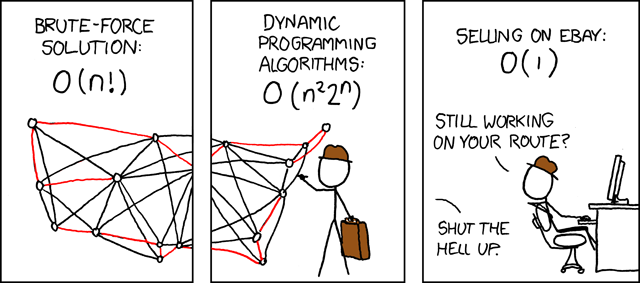
\includegraphics[scale=0.4]{tsp.png}
    \end{center}
\end{frame}

\begin{frame}[plain]{Top-down vs. bottom-up}
    \begin{itemize}
        \item What we have been doing so far is usually called top-down dynamic programming
        \item I.e. you start with the main problem (the top) and split it into smaller problems recursively (down)
        \item In some cases it can be better to do things bottom-up, which is pretty much just the reverse order
        \item Consider for example the fibonacci numbers. Then we'd start at the base cases and count up
    \end{itemize}
\end{frame}


\begin{frame}[plain]{Top-down vs. bottom-up}
    \begin{itemize}
        \item Bottom-up is generally faster, but it has the issue that we have to make sure we iterate through the sub problems in the right order, since recursion doesn't automatically handle that for us
        \item Then why would we use bottom-up?
        \item Sometimes knowing in what order we go through the states can be useful, let's take an example
    \end{itemize}
\end{frame}

\begin{frame}[plain]{Decelerating jump}
    \begin{itemize}
        \item Suppose we have $n$ squares in a row, each containing a value $a_i$. 
        \item We start at the first cell and want to jump through the cells.
        \item If we land on cell $i$ we get $a_i$ points and want to maximize our points.
        \item We can jump to any cell in front of us, but our jump can never go further than our last one.
        \item $n \leq 3000$, $-10^9 \leq a_i \leq 10^9$
    \end{itemize}
\end{frame}

\begin{frame}[plain]{Solution function}
    \begin{itemize}
        \item Let us then find a recursive function describing the answer. 
        \item Let $f(i, j)$ be the maximum score one can get starting at $i$ and using jumps of at most length $j$. Then
            \[f(i, j) = \begin{cases} a_n & \text{ if } i = n \\ \max\limits_{1 \leq k \leq \min(j, n - i)} f(i + k, k) + a_i & \text{ otherwise} \end{cases}\]
        \item Then we have $n^2$ states and it takes linear time to calculate each one. Thus a top-down solution would run in $\mathcal{O}(n^3)$, which is too slow.
    \end{itemize}
\end{frame}

\begin{frame}[plain]{Optimization}
    \begin{itemize}
        \item What about bottom up?
        \item Each $f(i, j)$ only depends on values of $f$ with greater $i$ and lesser $j$, so we can calculate them in increasing order of $j$ and decreasing order of $i$.
    \end{itemize}
\end{frame}

\begin{frame}[plain,fragile]{First implementation}
\scriptsize
\begin{minted}{cpp}
#define INF (1LL << 60)
int main() {
    ll n; cin >> n;
    ll d[n][n], a[n];
    for(int i = 0; i < n; ++i) cin >> a[i];
    for(int i = 0; I < n; ++i) for(int j = 0; j < n; ++j) d[i][j] = -INF;
    d[n - 1][1] = a[n - 1];
    for(int i = n - 2; i >= 0; --i) d[i][1] = d[i + 1][1] + a[i];
    for(int i = 0; i < n; ++i) d[n - 1][i] = a[n - 1];
    for(int j = 2; j < n; ++j) for(int i = n - 2; i >= 0; --i)
        for(int k = 1; k < min(j + 1, n - i); k++) 
            d[i][j] = max(d[i][j], d[i + k][k] + a[i]);
    cout << d[0][n - 1] << '\n';
}
\end{minted}
\end{frame}

\begin{frame}[plain]{Optimized?}
    \begin{itemize}
        \item This is still $\mathcal{O}(n^3)$, so still not good enough.
        \item We note that when we calculate $f(i, j)$ we use the maximum value along the diagonal $f(i + 1, 1), f(i + 2, 2), \dots, f(i + k, k)$.
        \item So we just add a prefix array for the diagonals to calculate those values in $\mathcal{O}(1)$.
        \item This will make the solution $\mathcal{O}(n^2)$, which is good enough, something that couldn't be done with top-down.
    \end{itemize}
\end{frame}

\begin{frame}[plain,fragile]{Fast implementation}
\scriptsize
\begin{minted}{cpp}
#define INF (1LL << 60)
int main() {
    ll n; cin >> n;
    ll d[n][n], e[n], a[n];
    for(int i = 0; i < n; ++i) cin >> a[i];
    for(int i = 0; I < n; ++i) for(int j = 0; j < n; ++j) d[i][j] = -INF;
    d[n - 1][1] = e[n - 1] = a[n - 1];
    for(int i = n - 2; i >= 0; --i) e[i] = d[i][1] = d[i + 1][1] + a[i];
    for(int i = 0; i < n; ++i) d[n - 1][i] = a[n - 1];
    for(int j = 2; j < n; ++j) {
        e[n - j] = max(e[n - j], d[n - 1][j] = a[n - 1]);
        for(int i = n - 2; i >= 0; --i) {
            d[i][j] = e[i + 1] + a[i];
            if(i >= j - 1) e[i - j + 1] = max(e[i - j + 1], d[i][j]);
        }
    }
    cout << d[0][n - 1] << '\n';
}
\end{minted}
\end{frame}

\begin{frame}[plain]{Subset sum problem}
    \vspace{10pt}

    \begin{itemize}
        \item Another common dynamic programming task is known as the subset sum problem. 
        
        \item Given $n$ positive integers $a_1, \dots, a_n$ find if there is a subset with sum $c$. Variants also include finding the sum closest to $c$, greatest sum not exceeding $c$ and so on.
        
        \item The naïve solution here would involve checking every subset, which if done efficiently (for example with gray codes) takes $O(2^n)$, which is quite slow.
    \end{itemize}
\end{frame}

\begin{frame}[plain]{Subset sum problem}
    \vspace{10pt}

    \begin{itemize}
        \item Let $f(i, s)$ be a boolean function answering whether there exists a subset of $a_1, \dots, a_i$ with sum $s$.
        
        \item Then      
        \[f(i, s) = \begin{cases}\texttt{true} \text{ if } i = s = 0 \\ \texttt{false} \text{ if } i = 0, s \neq 0 \\ \texttt{false} \text{ if } s < 0 \\ f(i - 1, s) \texttt{ or } f(i - 1, s - a_i) \text{ otherwise} \end{cases}\]
        
        \item The different variants can then be read from the values of $f$. Each state takes $O(1)$ to compute, and there are $n(a_1 + \dots + a_n)$ states. Denoting the sum by $\Sigma$ this makes our time complexity $O(n\Sigma)$, which isn't great, but is often better than $O(2^n)$.
    \end{itemize}
\end{frame}

\begin{frame}[plain,fragile]{Subset sum problem}
    \begin{minted}[fontsize=\scriptsize]{cpp}
const int N = 20;
const int SIGMA = 10000;
int a[N];
int dp[N][SIGMA]; 
// use int so -1 is unmemoized
// 0 and 1 are the bools as usual
bool subsetsum(int i, int s) {
    if(i < 0) return s == 0;
    if(s < 0) return false;
    if(dp[i][s] != -1) return dp[i][s];
    return dp[i][s] = subsetsum(i - 1, s) || subsetsum(i - 1, s - a[i]);
}
    \end{minted}
\end{frame}

\begin{frame}[plain]{Subset sum problem - variant}
    \vspace{10pt}

    \begin{itemize}
        \item Say we want to find the most even way to split the numbers into two groups, that is to say in a way that minimizes the difference of the sums of the two groups.
        
        \item Furthermore we want to actually output these numbers rather than just the difference in sum.
        
        \item We can use the subset sum solution to do this, simply adding a table that keeps track of what choices we made at what point.
    \end{itemize}
\end{frame}

\begin{frame}[plain,fragile]{Subset sum problem}
    \begin{minted}[fontsize=\scriptsize]{cpp}
#include<bits/stdc++.h>
using namespace std;
vector<int> a;
vector<vector<int>> dp, mv;
bool subsetsum(int i, int s) {
	if(i < 0) return s == 0;
	if(s < 0) return false;
    if(dp[i][s] != -1) return dp[i][s];
    dp[i][s] = 0;
    if(subsetsum(i - 1, s)) {
        dp[i][s] = 1;
        mv[i][s] = 1;
    } else if(subsetsum(i - 1, s - a[i])) {
        dp[i][s] = 1;
        mv[i][s] = 0;
    }
	return dp[i][s];
}
    \end{minted}
\end{frame}

\begin{frame}[plain,fragile]{Subset sum problem}
    \begin{minted}[fontsize=\scriptsize]{cpp}
int main() {
	int n, sm = 0; cin >> n;
	a = vector<int>(n);
	for(int i = 0; i < n; ++i)
		cin >> a[i], sm += a[i];
	dp = mv = vector<vector<int>>(n, vector<int>(sm, -1));
	int bst = sm / 2;
	while(!subsetsum(n - 1, bst)) bst--;
	vector<bool> group1(n, false);
	for(int i = n - 1; i >= 0; --i) {
		if(!mv[i][bst]) {
			group1[i] = true;
			bst -= a[i];
		}
	}
	cout << "Difference: " << abs(bst - (sm - bst)) << '\n';
	cout << "Group 1: ";
	for(int i = 0; i < n; ++i) if(group1[i]) cout << a[i] << ' ';
	cout << "\nGroup 2: ";
	for(int i = 0; i < n; ++i) if(!group1[i]) cout << a[i] << ' ';
	cout << '\n';
}
    \end{minted}
\end{frame}

\begin{frame}[plain]{Multidimensional DP comment}
    \vspace{10pt}

    \begin{itemize}
		\item The order in which you put the dimensions in a multidimensional dp can affect the running time.
		
		\item This is due to cache locality, so if you are fetching sequentially from one dimension and not the other, this can make one order faster.    
    
        \item Usually it doesn't matter, but in a few cases it might.
    \end{itemize}
\end{frame}

\begin{frame}[plain]{Knapsack problem}
    \vspace{10pt}

    \begin{itemize}
        \item The subset sum problem time complexity is exponential, as the sums of the numbers is exponential in the size of the actual input. 
        
        \item Among similar "hard" problems (in terms of time complexity) is the knapsack problem.
        
        \item We have $n$ items, each with some value and some weight. We also have a knapsack with a maximum weight capacity and want to maximize the value with respect to this condition.
    \end{itemize}
\end{frame}

\begin{frame}[plain]{Knapsack problem}
    \vspace{10pt}

    \begin{itemize}
        \item We can once more use dynamic programming to solve this.
        
        \item We let $f(i, j)$ be the maximum value we can get from the first $i$ items if our maximum weight is $j$.
       
       	\item Let $v_1, \dots, v_n$ be the values and $w_1, \dots, w_n$ the weights. Then 	
       	\[f(i, j) = \begin{cases}-\infty \text{ if } j < 0\\0 \text{ otherwise if } i = 0\\ \operatorname{max}(f(i - 1, j), f(i - 1, j - w_i) + v_i) \text{ otherwise}\end{cases}\]
       	\item The time complexity is then $O(nS)$ where $S$ is the sum of the weights.
       	\item We'll leave translating this into code as an exercise.
    \end{itemize}
\end{frame}

\begin{frame}[plain]{Egg dropping problem}
    \vspace{10pt}

    \begin{itemize}
        \item The previous problems are all very well known and classic in computer science. Let us also take a slightly less common example called the egg dropping problem.
        
        \item We have a building with $k$ floors and we wish to figure out from which floor we have to drop an egg so it breaks. I.e. for some $x$ dropping it from the $x$-th floor the egg will break, but dropping it from the $(x-1)$-st floor the egg won't break it.
        
        \item If we have $n$ eggs, how few trials can we get away with in the worst case?
    \end{itemize}
\end{frame}

\begin{frame}[plain]{Egg dropping problem}
    \vspace{10pt}

    \begin{itemize}
        \item Say we drop the egg from a floor $y$. 
        
        \item If the egg breaks, we only need to check floors $< y$ and have one less egg. This is essentially the same problem again but with $y - 1$ floors and $n - 1$ eggs.
        
        \item If the egg doesn't break we only need to check floors $> y$, so the problem is again the same with $k - y$ floors and $n$ eggs.
        
        \item Since we are looking at the worst case, our result is the worse of these two.
        
        \item Since we can choose any $y$, we take the best result among all $y$.
    \end{itemize}
\end{frame}

\begin{frame}[plain]{Egg dropping problem}
    \vspace{10pt}

    \begin{itemize}
        \item Let $f(n, k)$ be the minimum number of trials for $n$ eggs and $k$ floors. 
        \item We note that if we have one egg, we must always go through the floors in order since we can't afford to break an egg.
        \item All together this gives us
        \[f(i, j) = \begin{cases}1 \text{ if } k = 1 \\0 \text{ if } k = 0\\k \text{ if } i = 1\\ \min_{1 \leq x \leq k} 1 + \max(f(i - 1, x - 1), f(i, j - x))\end{cases}\]
        \item We see that this takes $O(k)$ per state and we have $O(nk)$ states, so the time complexity is $O(nk^2)$.
    \end{itemize}
\end{frame}

\begin{frame}[plain]{Egg dropping problem}
    \vspace{10pt}

    \begin{itemize}
        \item As a side note, this can also be solved in $O(nk)$ with a different dynamic programming approach.
        \item Try considering calculating the maximum number of floors you can check with $n$ eggs and $k$ trials using dynamic programming.
        
        \item Using some more clever ideas this can even be brought down to $O(n\log(k))$, but we won't need this here.
    \end{itemize}
\end{frame}

\begin{frame}[plain]{Complex states}
    \begin{itemize}
        \item Most problems so far have had a state representable with a fixed number of integer values.
        \item This has allowed us to use static arrays for memoization.
        \item What if the state is not easily representable by integers or parameters are dynamic in count?
        \item For example: a larger range of integers, a string, a vector, or a custom type
    \end{itemize}
\end{frame}

\begin{frame}[plain,fragile]{Complex states}
    \begin{minted}[fontsize=\scriptsize]{cpp}
map<vector<int32_t>, int32_t> mem;
int32_t dp(const vector<int32_t>& state) {
    vector<int32_t> next_state(state);
    int32_t result{ 0 };
    for (auto& x : next_state) {
        if (x > 0) {
            int32_t old = x;
            x /= 2;
            result += dp(next_state);
            x = old;
        }
    }
    return result;
}
    \end{minted}
\end{frame}

\begin{frame}[plain,fragile]{Complex states}
    \begin{minted}[fontsize=\scriptsize]{cpp}
map<tuple<type1_t, type2_t, ...>, result_t> mem;
// alternatively use unordered_map, need to ensure state is hashable
result_t dp(type1_t param1, type2_t param2, ...) {
    const auto state{ tie(param1, param2, ...) };
    if (is_base_case(state)) {
        return 0; // or 1 or whatever it should be
    }
    if (const auto it{ mem.find(state) }; it != mem.end()) {
        return it->second;
    }
    result_t result{};
    // compute answer recursively
    return mem[state] = result;
}
    \end{minted}
\end{frame}

\end{document}
